\documentclass[a4paper,5pt]{amsbook}
%%%%%%%%%%%%%%%%%%%%%%%%%%%%%%%%%%%%%%%%%%%%%%%%%%%%%%%%%%%%%%%%%%%%%

\usepackage{booktabs}
\usepackage{graphicx}
\usepackage{multicol}
\usepackage{textcomp}
\usepackage{systeme}
\usepackage{amssymb}
\usepackage[]{amsmath}
\usepackage{subcaption}
\usepackage[inline]{enumitem}
\usepackage{gensymb}

%%%%%%%%%%%%%%%%%%%%%%%%%%%%%%%%%%%%%%%%%%%%%%%%%%%%%%%%%%%%%%

\newcommand{\sen}{\,\mbox{sen}}
\newcommand{\tg}{\,\mbox{tg}\,}
\newcommand{\cosec}{\,\mbox{cosec}\,}
\newcommand{\cotg}{\,\mbox{cotg}\,}
\newcommand{\tr}{\,\mbox{tr}\,}
\newcommand{\ds}{\displaystyle}
\newcommand{\ra}{\rightarrow}

%%%%%%%%%%%%%%%%%%%%%%%%%%%%%%%%%%%%%%%%%%%%%%%%%%%%%%%%%%%%%%%%%%%%%%%%

\setlength{\textwidth}{16cm} %\setlength{\topmargin}{-1.3cm}
\setlength{\textheight}{25cm}
\setlength{\leftmargin}{1.2cm} \setlength{\rightmargin}{1.2cm}
\setlength{\oddsidemargin}{0cm}\setlength{\evensidemargin}{0cm}

%%%%%%%%%%%%%%%%%%%%%%%%%%%%%%%%%%%%%%%%%%%%%%%%%%%%%%%%%%%%%%%%%%%%%%%%

% \renewcommand{\baselinestretch}{1.6}
% \renewcommand{\thefootnote}{\fnsymbol{footnote}}
% \renewcommand{\theequation}{\thesection.\arabic{equation}}
% \setlength{\voffset}{-50pt}
% \numberwithin{equation}{chapter}

%%%%%%%%%%%%%%%%%%%%%%%%%%%%%%%%%%%%%%%%%%%%%%%%%%%%%%%%%%%%%%%%%%%%%%%

\begin{document}
\thispagestyle{empty}
\pagestyle{empty}
\begin{minipage}[h]{0.14\textwidth}
	
\includegraphics[scale=0.24]{../../ufgd.png}
\end{minipage}
\begin{minipage}[h]{\textwidth}
\begin{tabular}{c}
{{\bf UNIVERSIDADE FEDERAL DA GRANDE DOURADOS}}\\
{{\bf C\'alculo de V\'arias Vari\'aveis --- Lista 1}}\\
{{\bf Prof.\ Adriano Barbosa}}\\
\end{tabular}
\vspace{-0.45cm}
%
\end{minipage}

%------------------------

\vspace{1cm}
%%%%%%%%%%%%%%%%%%%%%%%%%%%%%%%%   formulario  inicio  %%%%%%%%%%%%%%%%%%%%%%%%%%%%%%%%
\begin{enumerate}
    \setlength\itemsep{0.5cm}
    \item Um modelo para o c\'alculo da \'area da superf\'{\i}cie do corpo humano \'e dado
    pela fun\c{c}\~ao $A=f(w,h)=0,1091w^{0,425}h^{0,725}$, onde $w$ \'e o peso (em
    libras), $h$ \'e a altura (em polegadas) e $A$ \'e a \'area medida em p\'e
    quadrado.
        \begin{enumerate}
            \setlength\itemsep{0.2cm}
            \item Calcule $f(160,70)$ e interprete o resultado.
            \item Qual a \'area da superf\'{\i}cie do seu corpo?
        \end{enumerate}
        \vspace{0.2cm}
        (1 libra = 0,453 kg, 1 polegada = 0,0254 m e 1 p\'e quadrado = 0,093 m$^2$)

%    \item Seja $g(x,y)=\cos(x+2y)$.
%        \begin{enumerate}
%            \setlength\itemsep{0.2cm}
%            \item Calcule $g(2,-1)$.
%            \item Determine o dom\'{\i}nio de $g$.
%            \item Determine a imagem de $g$.
%        \end{enumerate}

    \item Encontre o dom\'{\i}nio das fun\c{c}\~oes:

        \begin{enumerate*}
            \item $f(x,y) = \sqrt{2x-y}$
            \hspace{0.5cm}
            \hspace{0.5cm}
            \item $f(x,y) = \ln{9-x^2-9y^2}$
            \hspace{0.5cm}
            \hspace{0.5cm}
            \item $f(x,y) = \ds\frac{\sqrt{y-x^2}}{1-x^2}$
        \end{enumerate*}

    \item Desenhe o gr\'afico das fun\c{c}\~oes:

        \begin{enumerate*}
            \item $f(x,y) = 1+y$
            \hspace{0.5cm}
            \hspace{0.5cm}
            \item $f(x,y) = 10-4x-5y$
            \hspace{0.5cm}
            \hspace{0.5cm}
            \item $f(x,y) = 9-x^2-9y^2$
        \end{enumerate*}

    \item Identifique as fun\c{c}\~oes com seus gr\'aficos:

    \begin{minipage}[r]{0.4\textwidth}
        \begin{enumerate}
            \setlength\itemsep{0.2cm}
            \item $f(x,y) = |x|+|y|$
            \item $f(x,y) = |xy|$
            \item $f(x,y) = \ds\frac{1}{1+x^2+y^2}$
            \item $f(x,y) = (x^2-y^2)^2$
            \item $f(x,y) = (x-y)^2$
            \item $f(x,y) = \sen(|x|+|y|)$
        \end{enumerate}
    \end{minipage}
    \hfill{}
    \begin{minipage}[l]{0.5\textwidth}
        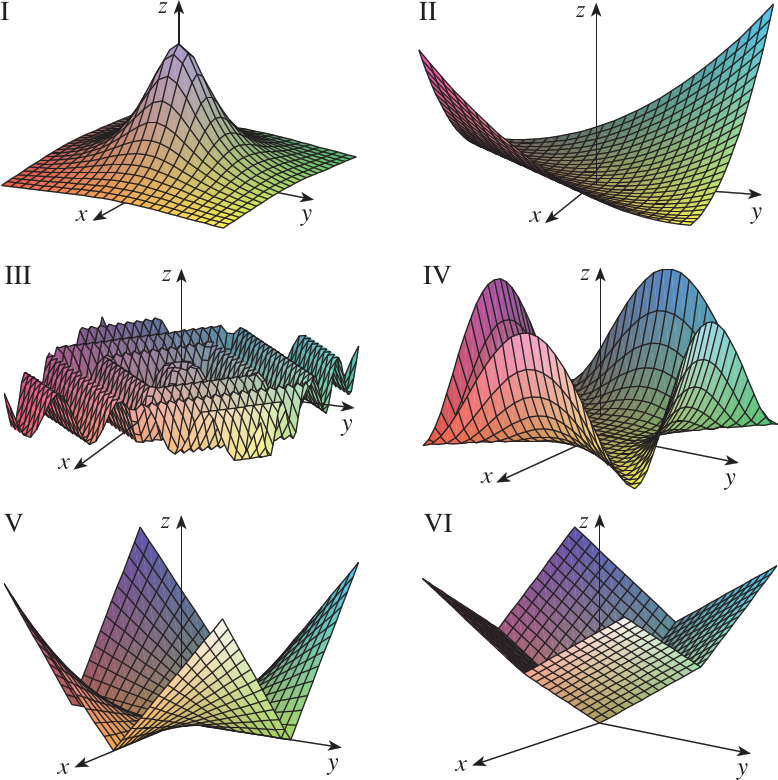
\includegraphics[width=\textwidth]{lista-01-fig1.png}
    \end{minipage}

    \item Use o mapa de contorno de $f$ para estimar os valores de $f(-3,3)$ e $f(3,-2)$.
        \begin{figure}[h]
            \centering
            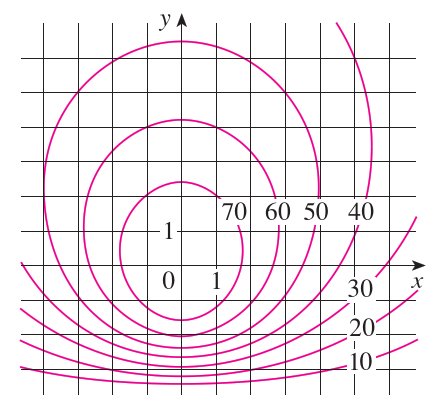
\includegraphics[width=0.3\textwidth]{lista-01-fig2.png}
        \end{figure}
\end{enumerate}

\end{document}
